\documentclass[epsfig]{article}
\usepackage{epsfig}
\usepackage{amsmath}
\usepackage{verbatim}
\usepackage{booktabs}
\usepackage{subfig}
\usepackage{graphicx}
\usepackage[english]{babel}
\usepackage{float}
\textwidth 6.7in
\oddsidemargin -0.1in
\textheight 8.50in
\topmargin -0.55in
\renewcommand{\textfraction}{0.25}
\renewcommand{\floatpagefraction}{0.7}
\markboth{}{\sl E. Mer\'enyi \hfil COMP / ELEC / STAT 502 \hfil Homework 4 }
\pagestyle{myheadings}
\def\bpar{\vskip26pt}
\def\npar{\vskip13pt}
\def\spar{\vskip10pt}
\begin{document}
\parindent=0pt
\null
{\bf 
\npar
Zhuo Chen, Yidan Pan

Equally contributed
\bpar
}

\bpar
\centerline{\bf Homework 4}
\npar

{\bf 
\npar
a Report network parameters
\bpar
}

\begin{table}[htbp] 
\center
\caption{Parameters of Training BP Network to Fit $f(x) = 1/x$}
  \label{tab:NP}
  %\scalebox{0.9}{ % You can scale the size of the table by changing this number
   \scalebox{1.0}{
   \begin{tabular}{p{4cm} p{.05cm} p{8cm}}
\toprule
  \multicolumn{3}{l}{\bf Network parameters} \\
\bottomrule \noalign{\smallskip}
  Topology & & $(1 + 1_{Bias})$ --- $(10 )$ --- $1$ \\
  Transfer function & & tanh with slope of 1 \\
\toprule
  \multicolumn{3}{l}{\bf Learning parameters} \\
\bottomrule \noalign{\smallskip}
  Initial weights & & drawn from U[-0.1, 0.1] \\
  Learning rate ($\alpha$) & & 0.01 \\
  Momentum & & none\\
  Epoch size ($Epoch$)& &  200 \\
  Stopping criteria & &  error ($Err_{RMSD}$) $ \le 0.05 $ OR  learn count (t) $ > 4,000,000 $\\
  Error measure($Err_{RMSD}$) & &  Square root of the sum of $(D-y)^2$ that averaged over all training or testing samples (see formula (1) below)\\\toprule
 \multicolumn{3}{l}{\bf Input / output data, representation, scaling} \\
\bottomrule \noalign{\smallskip}
  \# training samples ($N_{tr}$)& & 200 (x values drawn randomly from U[0.1,1])\\
  \# test samples ($N_{tst}$)& & 100 (x values drawn randomly from U[0.1,1])\\
  Scaling of inputs & &  no scaling \\
  Scaling of outputs & &  map [global min, global max] to [-1,1] \\

 \bottomrule \noalign{\smallskip}
 
  \end{tabular}
   } % end scalebox
\end{table}

The formula of the error we computed is:

$$(1)\ \ \ Err_{RMSD}= \sqrt{{1\over{|X|}}\sum_{k=1}^{|X|}(D^k-y^k)^2}$$

Where $k$ is the sample index, $X$ is either the whole training or testing data set at a particular learn count. Based on the parameter we used, The size of $X$ is constant: 200 for training set, 100 for testing set.
\spar
\spar
\spar
\spar
{\bf 
\npar
c Plot performance indicator of the network
\bpar
}
We use $Err_{RMSD}$(RMSE) as the performance indicator. The formula is shown as above. The figure shows the RMSE of training set. The RMSE is calculated every 10000 steps(50x200, where 200 is the size of training input set). We saw that  two spikes appeared in the process.

\begin{figure}[!htb] 
\centering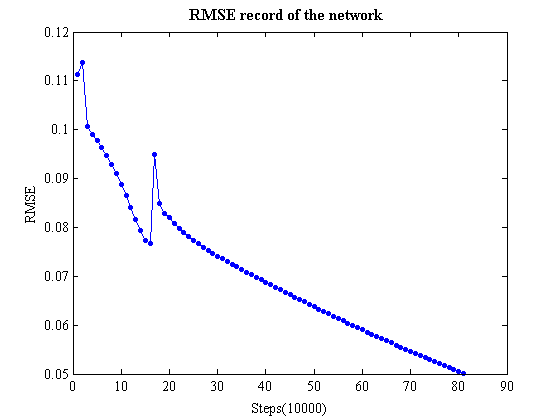
\includegraphics[width=4.5in]{fig1.png} 
\end{figure} 

\spar

After that, we compared the actual output with desired output after training is finished. The data is shown in the figure below:

\begin{figure}[!htb] 
\centering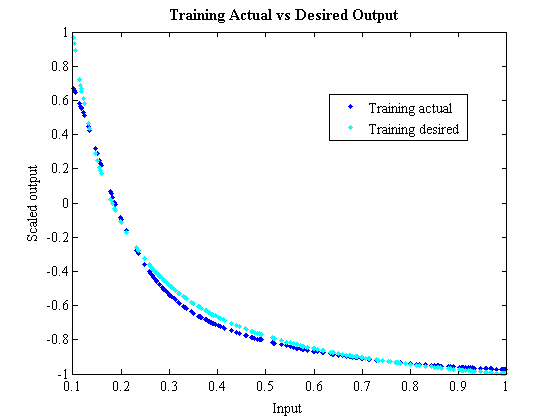
\includegraphics[width=4in]{fig2.png} 
\end{figure} 



The desired output vs actual output. The actual output is shown in blue and the desired output is shown in  In this run, 812400 steps were taken to make the final RMSE not higher than 0.05 (the average error we accept is 2.5\%).

{\bf 
\npar
d Number of learning step
\bpar
}

We set the criteria as RMSE $\le$ 0.05 or number of step exceeds 4,000,000. After running the script using the parameters given above for 20 times, the average steps for achieving RMSE $\le$ 0.05 is 756620, while the standard deviation is 203769. Though the minimum required step is good, further optimization on the parameters is required to generate a more stable learning network.
 \spar

{\bf 
\npar
e Training accuracy
\bpar
}
The figure showed below compared the RMSE of test set and training set per each 10000 steps (50x200, where 200 is the size of training input set). The RMSE of testing set are shown in red, and the RMSE of training set are shown in blue. The RMSEs of test set in large step number are even lower than the training set.

It is one thing that need to be highlighted that there are actually 50 training runs interval between each point in the figure. For training set, each run goes through 200 samples, and these will be 10000 steps. For test set, each run goes through 100 samples, and these will be 5000 steps. 
 \spar
{\bf Note: Here 1 step means 1 sample being taken into the training, so 1 epoch=200 steps (which made the count of steps a huge number).} 

 \begin{figure}[!htb] 
\centering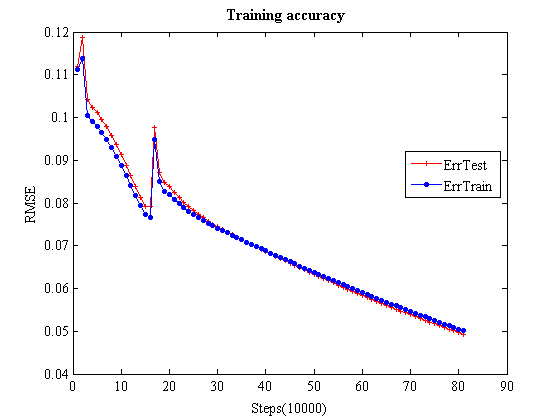
\includegraphics[width=4.5in]{fig3.png} 
\end{figure} 

After training is finished, the actual vs desired output for all points of both the training and testing data set is shown in the figure below:

\begin{figure}[!htb] 
\centering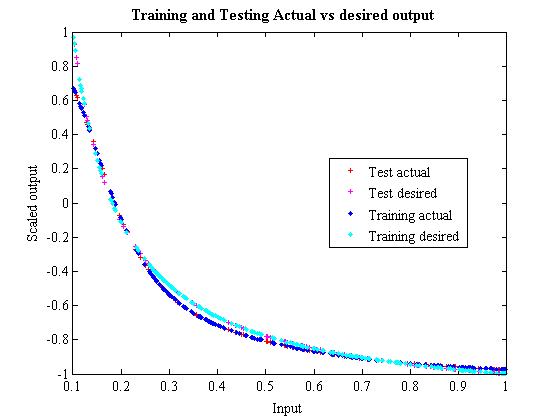
\includegraphics[width=4.5in]{fig4.png} 
\end{figure} 

It is clear that the two curves formed by the actual outputs coincide, though the points do not coincide in general. The same pattern is shown in the two curves formed by the desired outputs of training set and testing set. This data indicates that the recall ability of this net work is pretty good.

{\bf 
\npar
f Increasing the steps
\bpar
}
 
We also tried to increase the number of steps. During training for 20,000 cycles, the changing of RMSE of both training set and test set are shown in the figure below:

\begin{figure}[!htb] 
\centering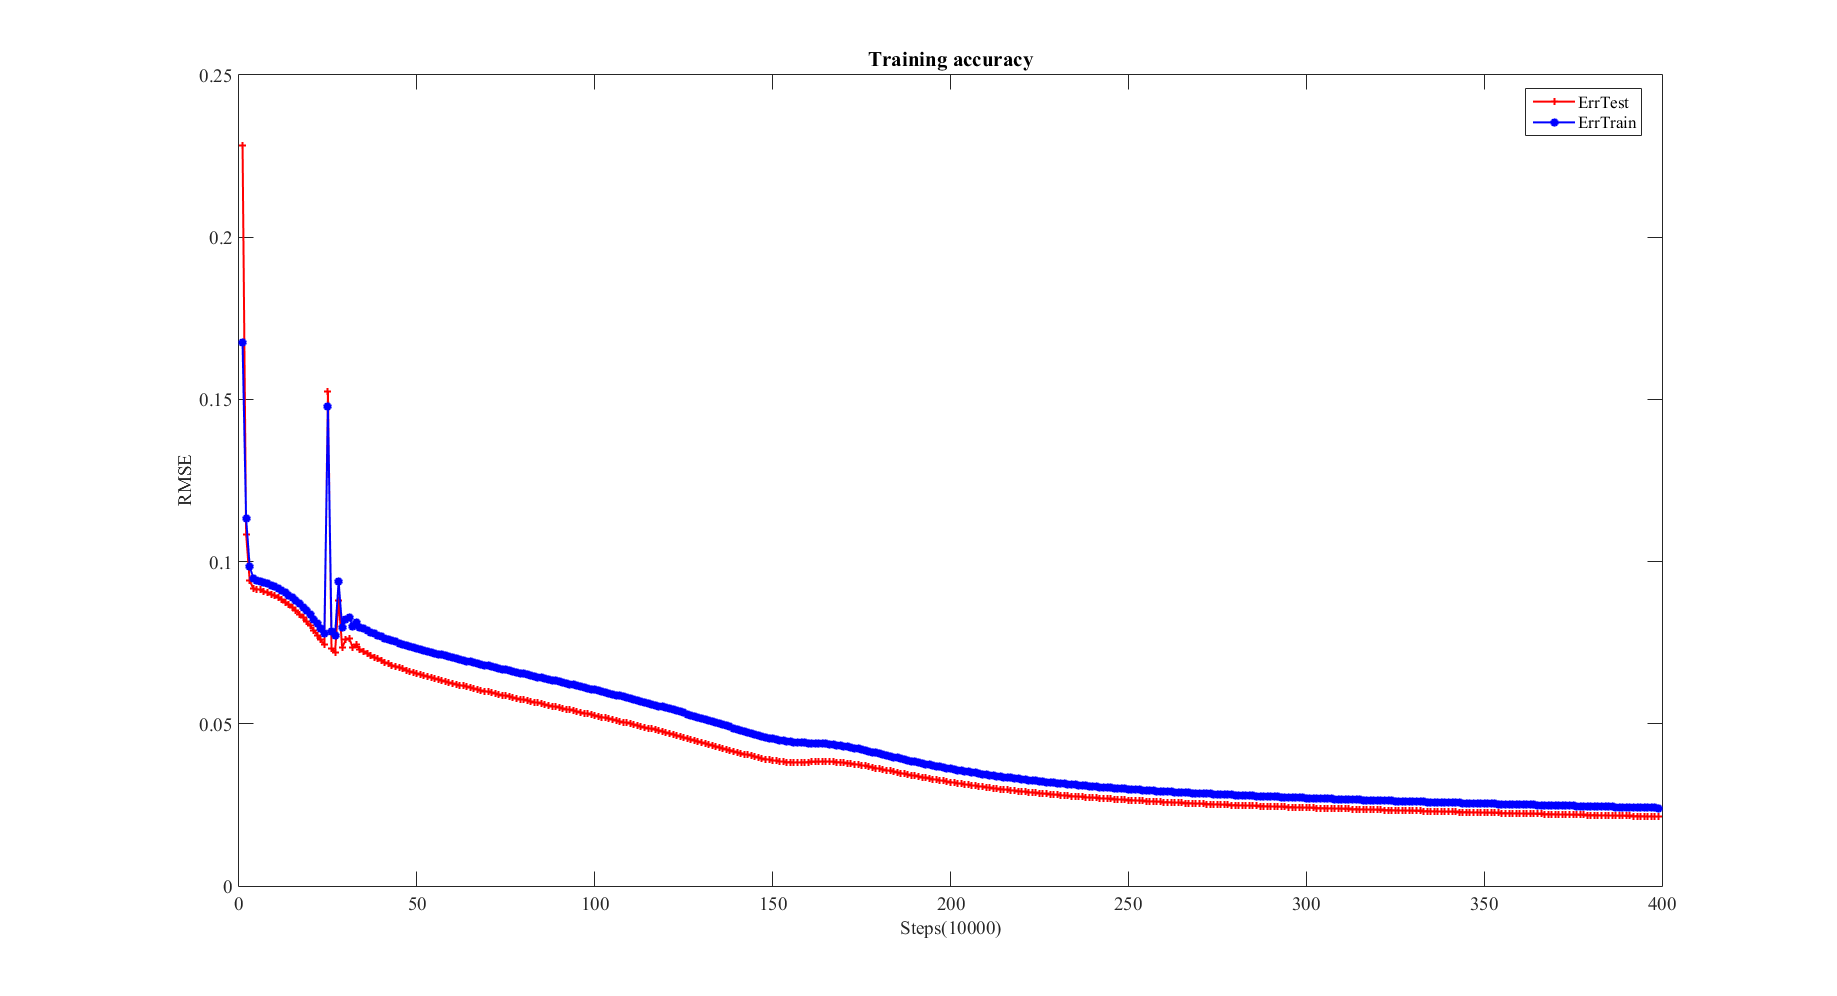
\includegraphics[width=6in]{fig5.png} 
\end{figure} 

The final RMSE of testing set is 0.0214, and the final RMSE of training set is 0.0237. We tried multiple times, and all the trends are similar: we saw some spikes at the very beginning, and then the error rate decreases and becomes flat.
\spar
The figure below compared the output pair of testing set and training set. From this we can see that while the general pattern are similar, the fitting is better than the one we performed above.
\begin{figure}[!htb] 
\centering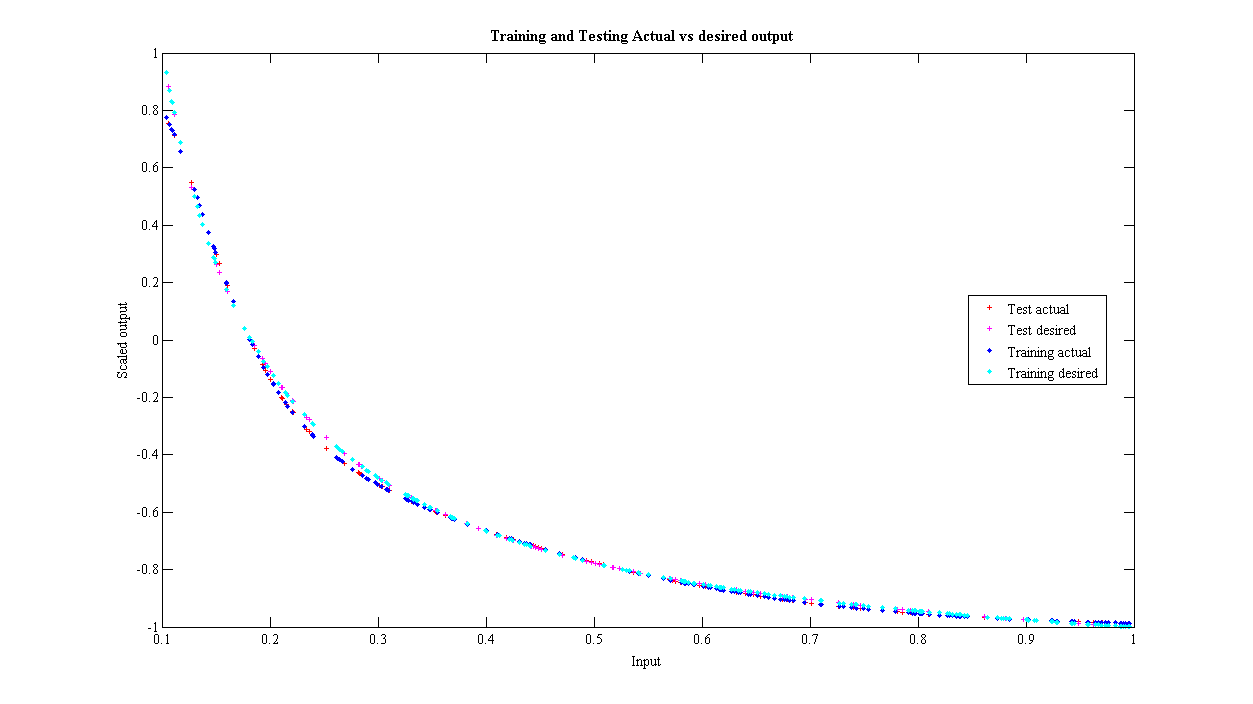
\includegraphics[width=6in]{fig6.png} 
\end{figure} 
 
 %{\bf 
%\npar
%g Trying different learning rate in two layers
%\bpar
%}
% 
%We tried to see if using different learning rate in different layers will generate better result. However, we have not finished the scanning.
 
\end{document}